\chapter{Software Design}
\label{chapter:software-design}

\section{Domain Model Diagram}
Det første skridt i designprocessen er at lave et Domain Model Diagram (DMD). Det er vigtigt at bemærke følgende:
\begin{itemize}
    \item DMD forholder sig til den virkelige verdens koncepter og relationer
    \item DMD er en statisk model, der ikke tager højde for ændringer i systemet over tid
    \item DMD anvender \emph{entities} til at repræsentere konceptuelle klasser
    \item DMD anvender \emph{relations} til at vise, hvordan \emph{entities} er relateret til og interagere med hinanden på et konceptuelt plan
    \item DMD kan bruges til at skabe en fælles forståelse af projektet og identificere de vigtigste klasser og \emph{relations}
    \item DMD kan bruges til at skabe en bedre forståelse af problemet for udviklerne og dermed en bedre løsning
    \item DMD kan bruges til at identificere de vigtigste klasser og deres \emph{relations}
    \item DMD er ikke en teknisk model og kan ikke direkte implementeres i software
\end{itemize} 
Kontrast skal primært ses i forhold til et Domain Class Diagram, hvor hver klasse har attributter, metoder og er forbundet andre klasser gennem specificerede relationer (fx agrregation) og mulitplicitet. 
Ligeledes ville man i et DCD se klasserne Basket, BasketItem og BasketSerice, muligvis med et IBasketService interface som implementeringen af konceptet "Kurv".
Det er vigtigt at definere ovenstående, da DMD er et godt værktøj men der er for mange holdninger til hvad det egentlig er.
\begin{figure}
    \centering
    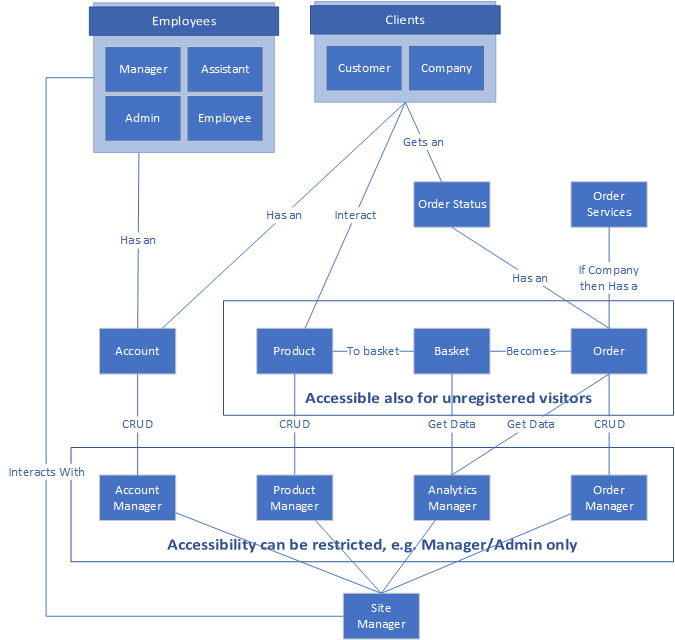
\includegraphics[width=0.8\textwidth]{figures/diagrams/dmd-start.png}
    \caption{Domain Model Diagram ved projektets start}
    \label{fig:domain-model-diagram}
\end{figure}

\section{Software Arkitektur}
Visse dele af denne section, er gennemgået i \Cref{sec:metode-teknologi} og yderligere beskrevet og argumenteret for i \Cref{chapter:anvendte-teknologier}. 
For fælles forståelse, vil software arkitektur i denne rapport forståes som; En højniveau beskrivelse af systemet, der beskriver dets komponenter, deres relationer og hvordan de interagerer. Derfor er den overordnede hensigt og struktur, som følger:
\begin{itemize}
    \item Abstraktioner af systemet, der fokuserer på dets struktur og adfærd
    \item En statisk model, der ikke tager højde for ændringer i systemet over tid
    \item Ligeledes en teknisk model, der kan bruges som blueprint til implementation
    \item Skabe en fælles forståelse af projektet og identificere de vigtigste komponenter og relationer
    \item Software arkitektur som koncept, kan bruges til at skabe en bedre forståelse og forudsigelse af problemeer for udviklerne og dermed en bedre løsning til tiden
\end{itemize}

\subsection{Klasse Diagram}
Et \emph{Design Class Diagram} vil i denne sammenhæng være arbejdstegninger for kernen af systemet. Det vil illustrere relationerne mellem de klasser, som systemet vil instansiere objekter ud fra og deres underlæggende properties og methods. 
Dette er for at skabe en forståelse for systemet. Dermed er det også et bevidst valg, ikke at meddrage PageModels og deres Views. Dette er grundet, at deres antal og relationer vil obfuskere overblikket, fremfor at fremme forståelse. 
Dette ses som værende den dimentralt modsatte hensigt med et diagram. Ligeledes er diagrammerne delt op i fire kategorier, for netop at bevare overblikket over systemet.
\begin{figure}
    \centering
    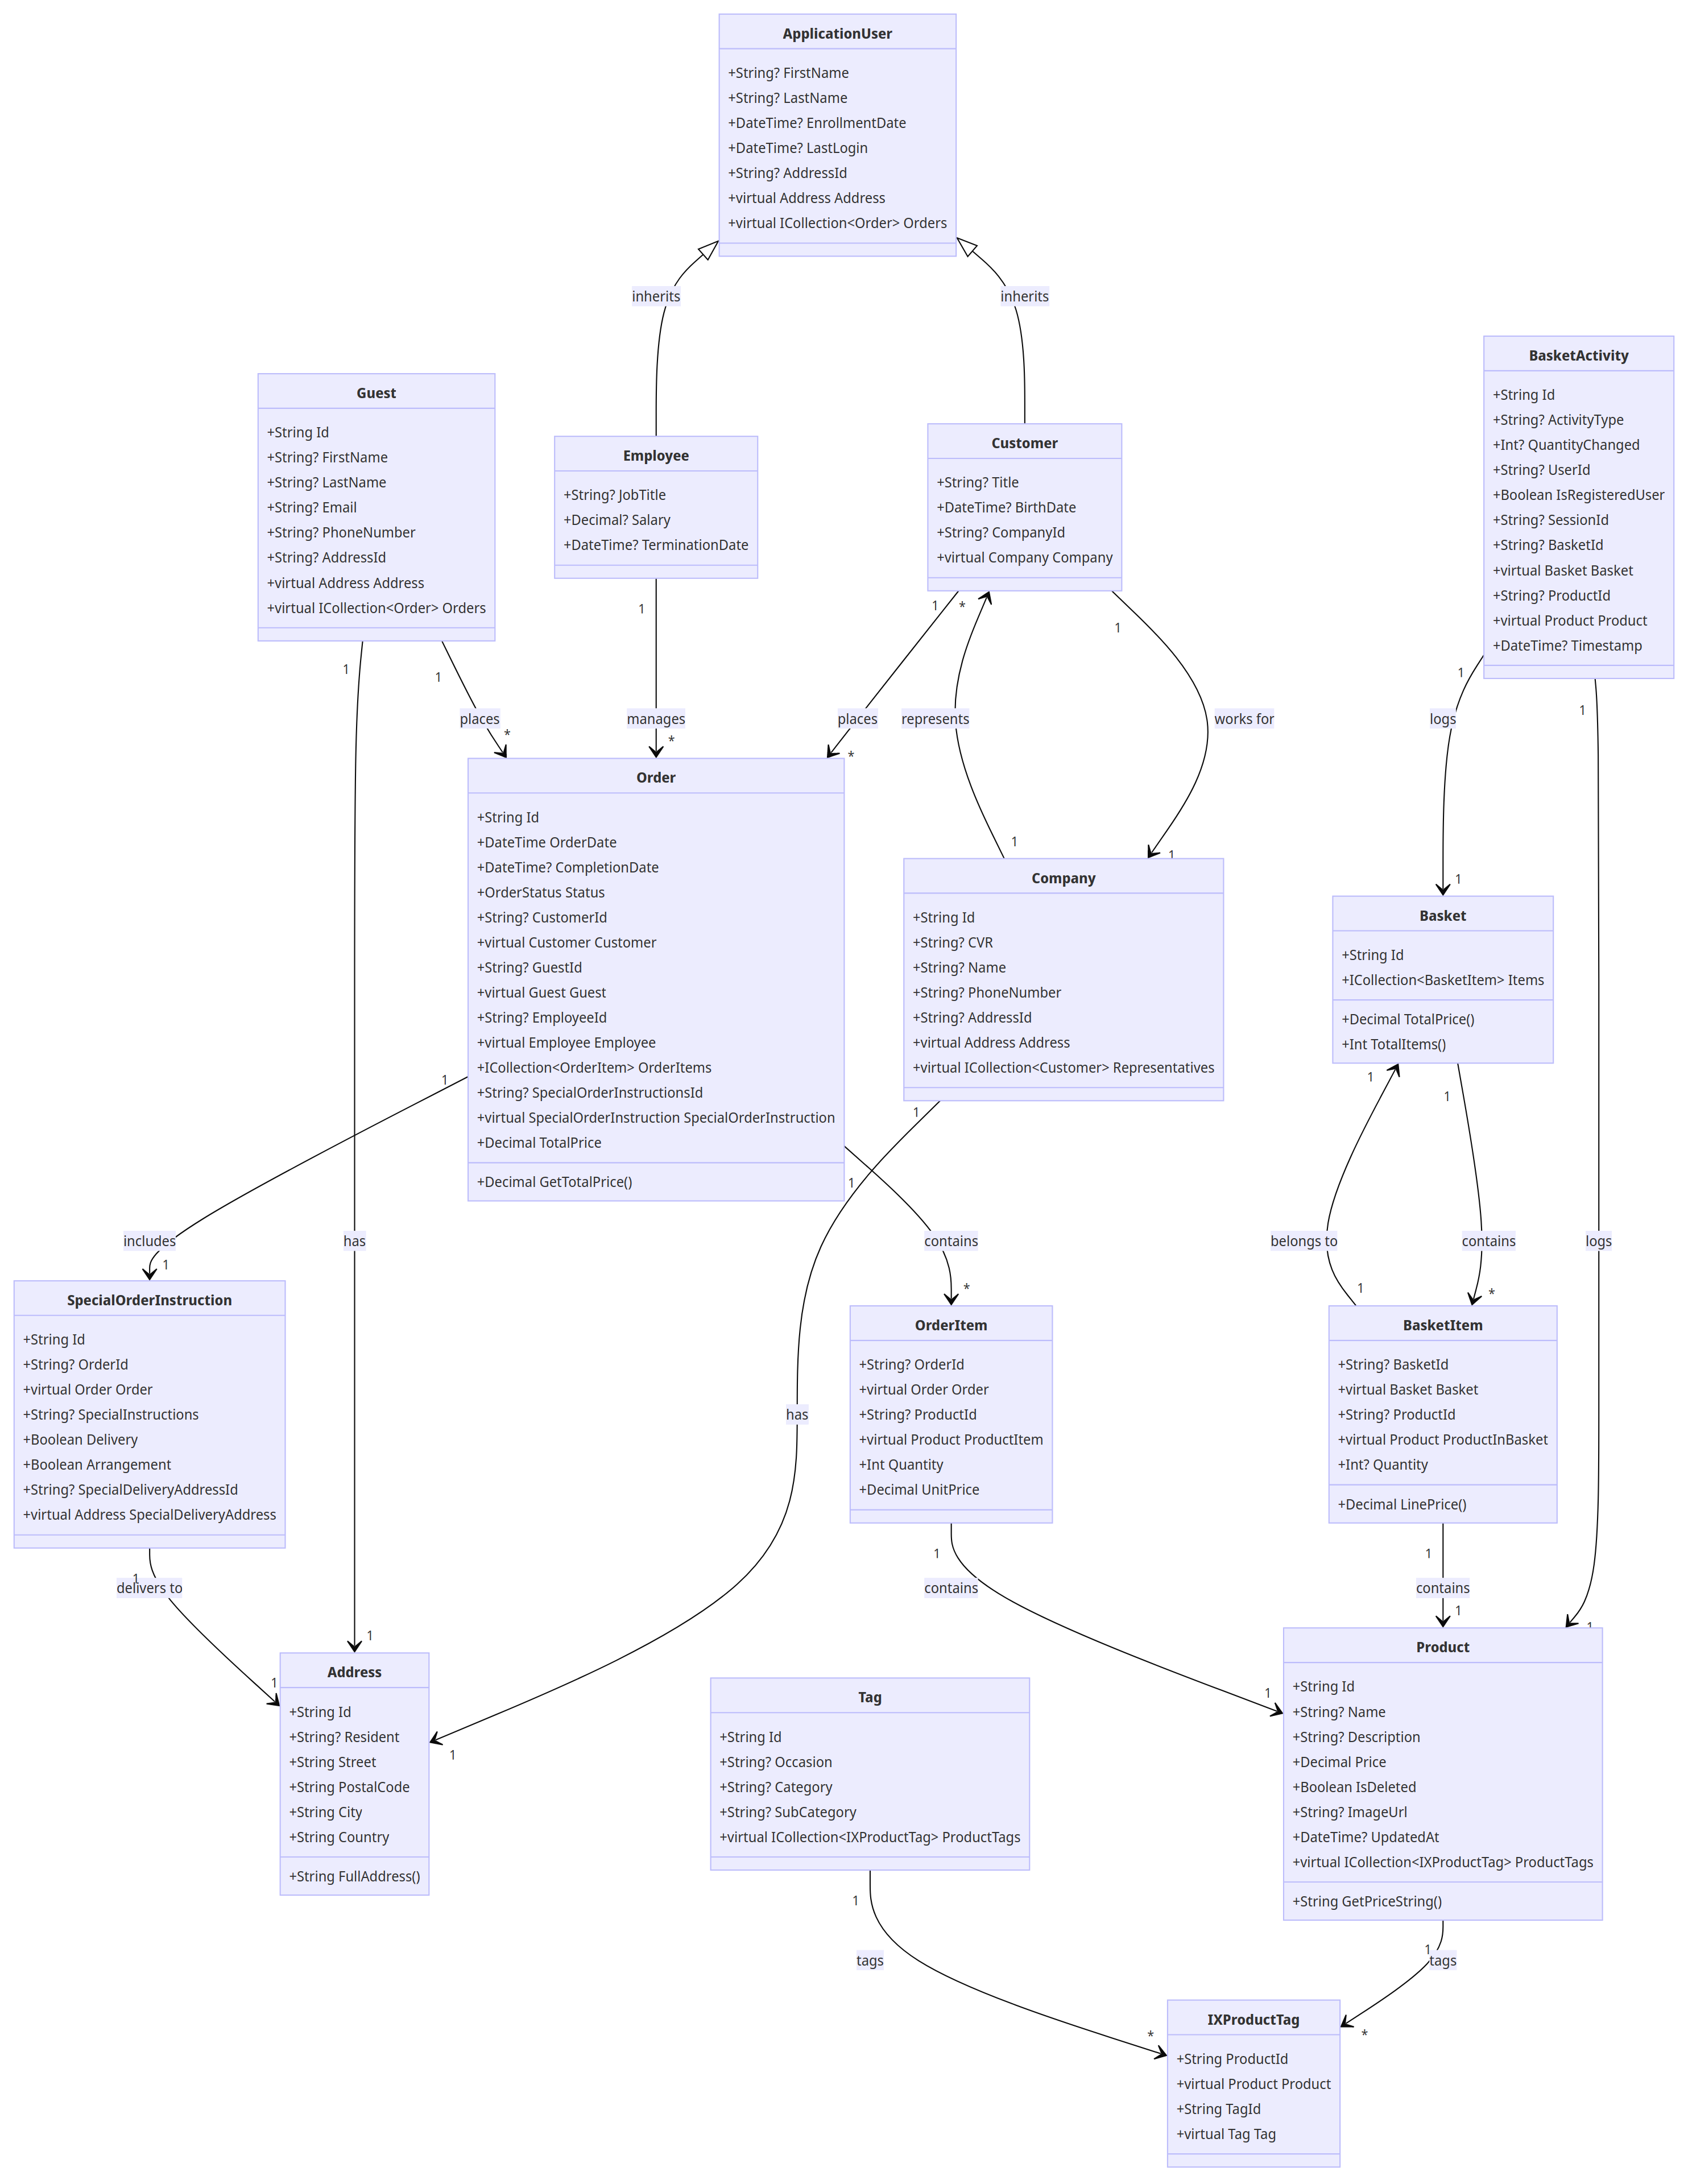
\includegraphics[width=0.8\textwidth]{figures/diagrams/dcd-modelclasses.png}
    \caption{Design Class Diagram - Model Classes}
    \label{fig:class-diagram-models}
\end{figure}

\begin{figure}
    \centering
    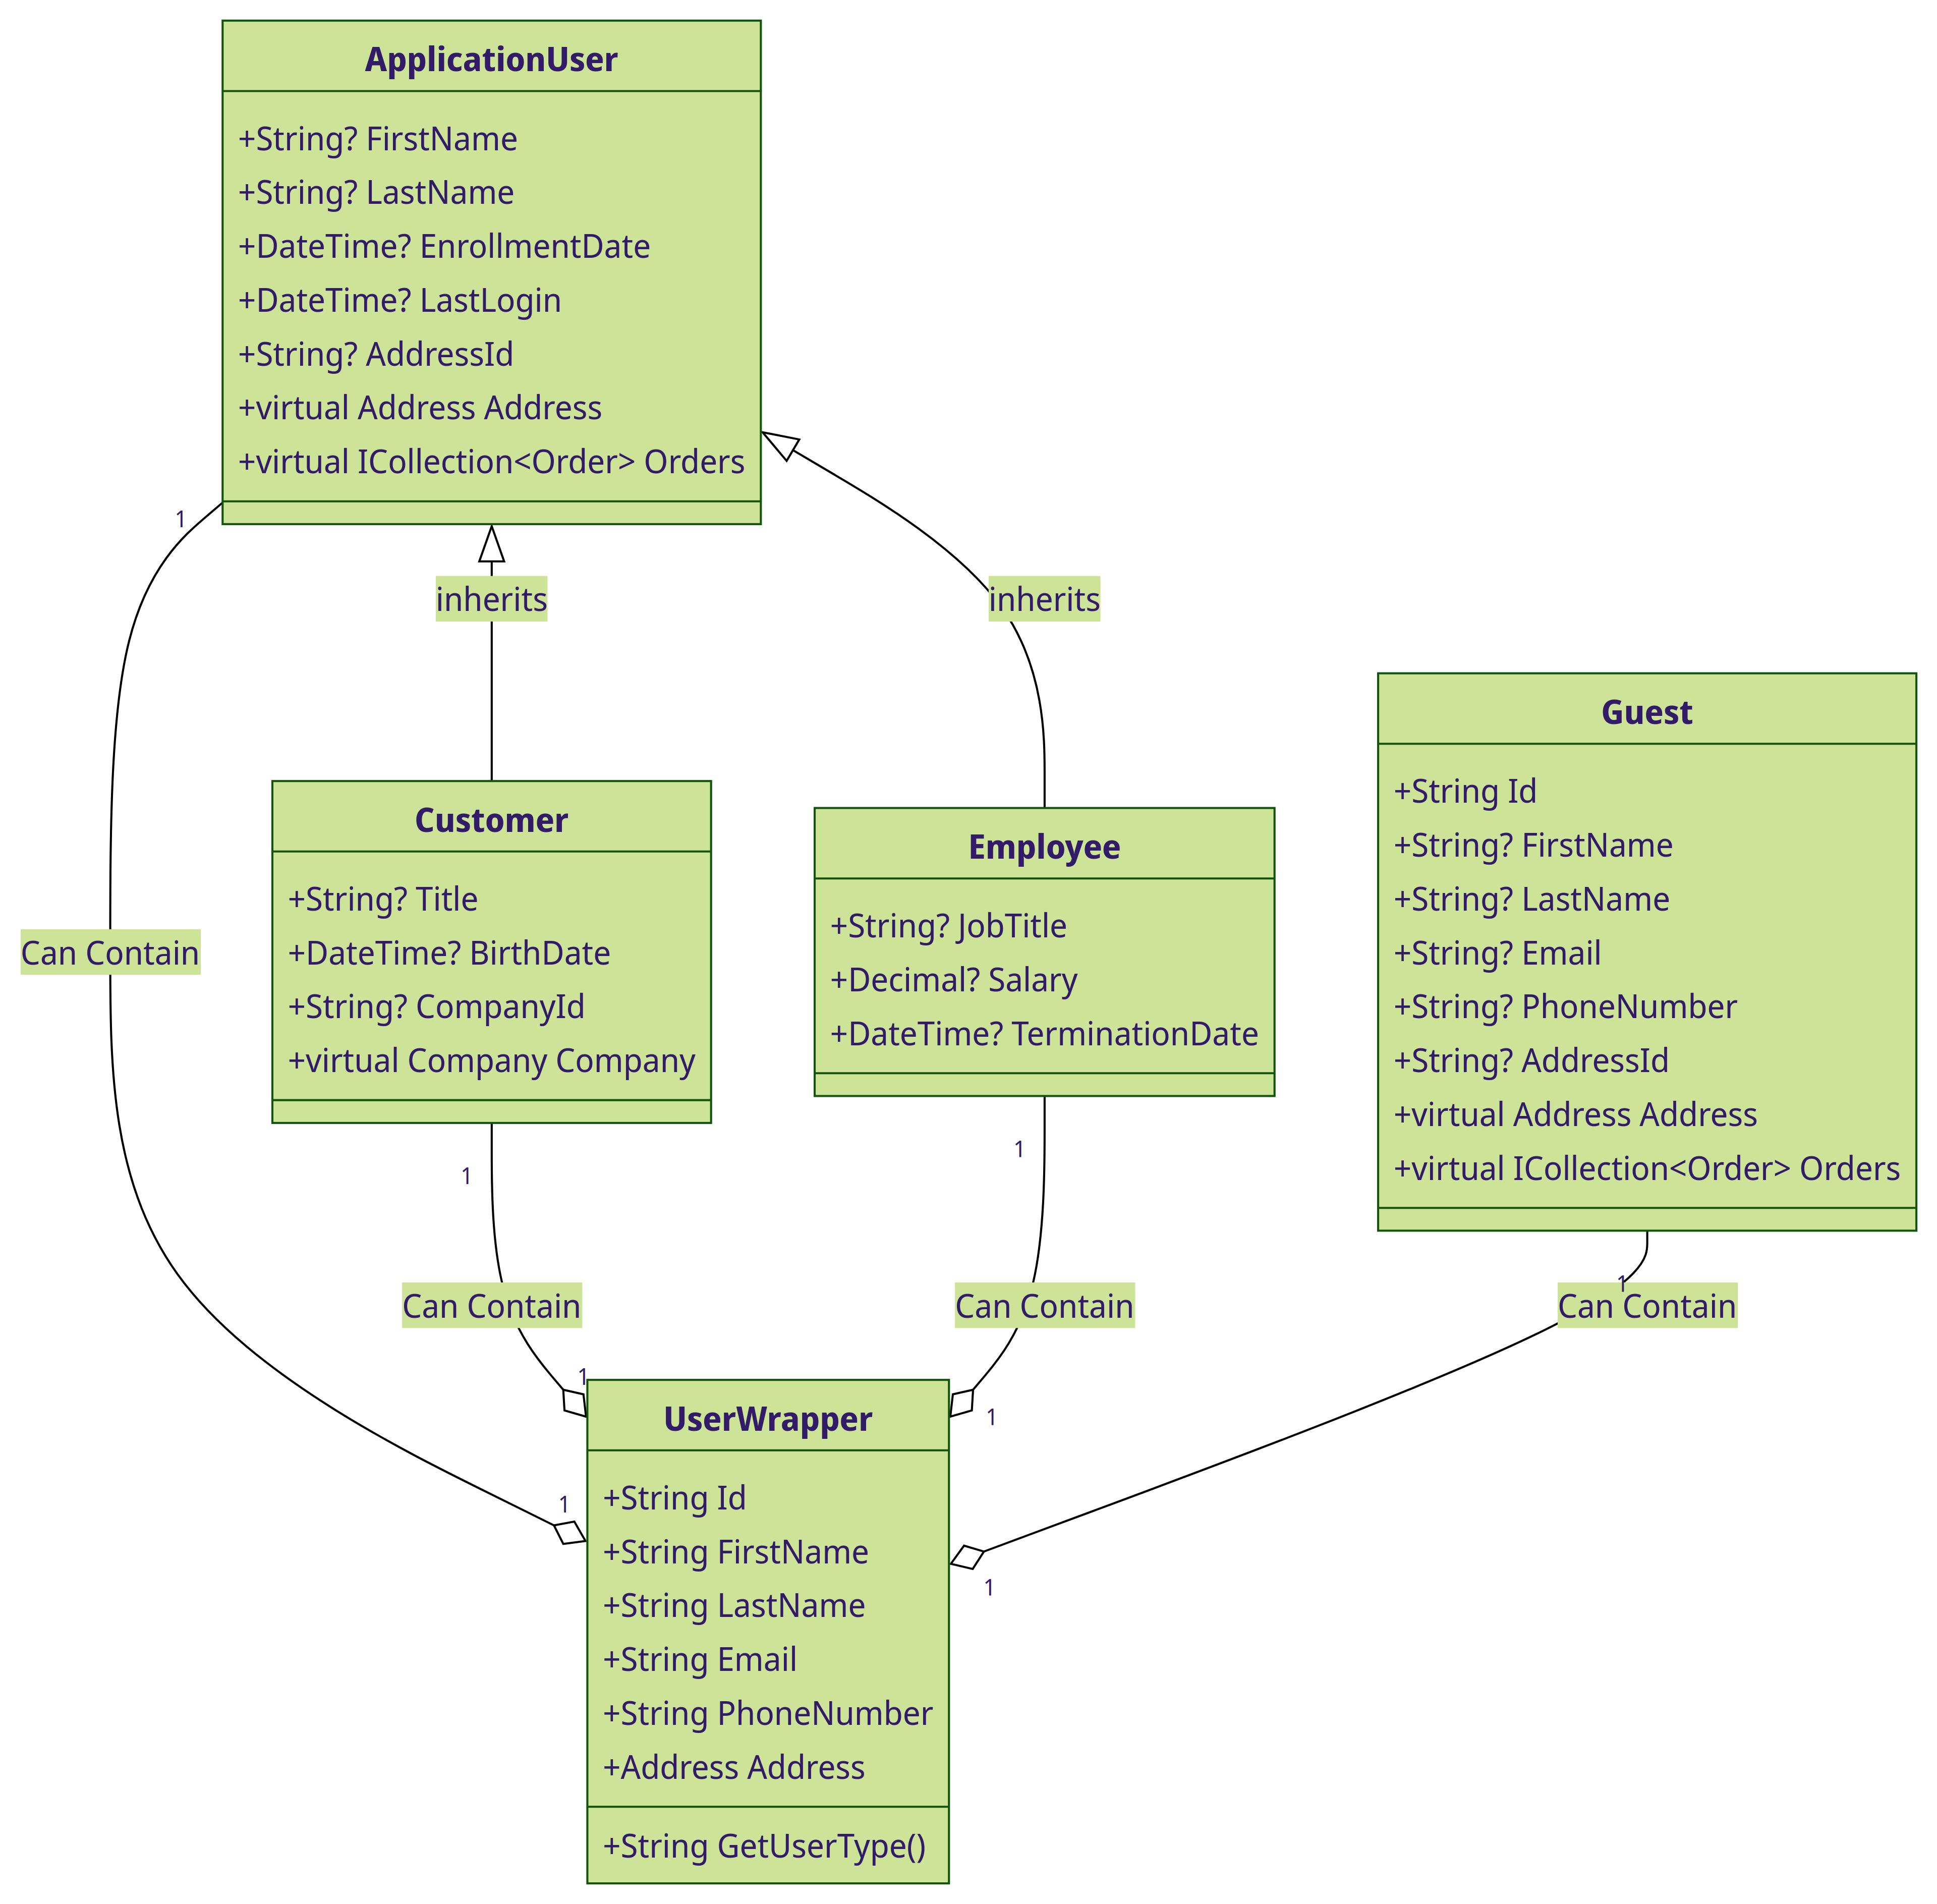
\includegraphics[width=0.8\textwidth]{figures/diagrams/dcd-user-userwrapper.png}
    \caption{Design Class Diagram - UserWrapper}
    \label{fig:class-diagram-userwrapper}
\end{figure}

\begin{figure}
    \centering
    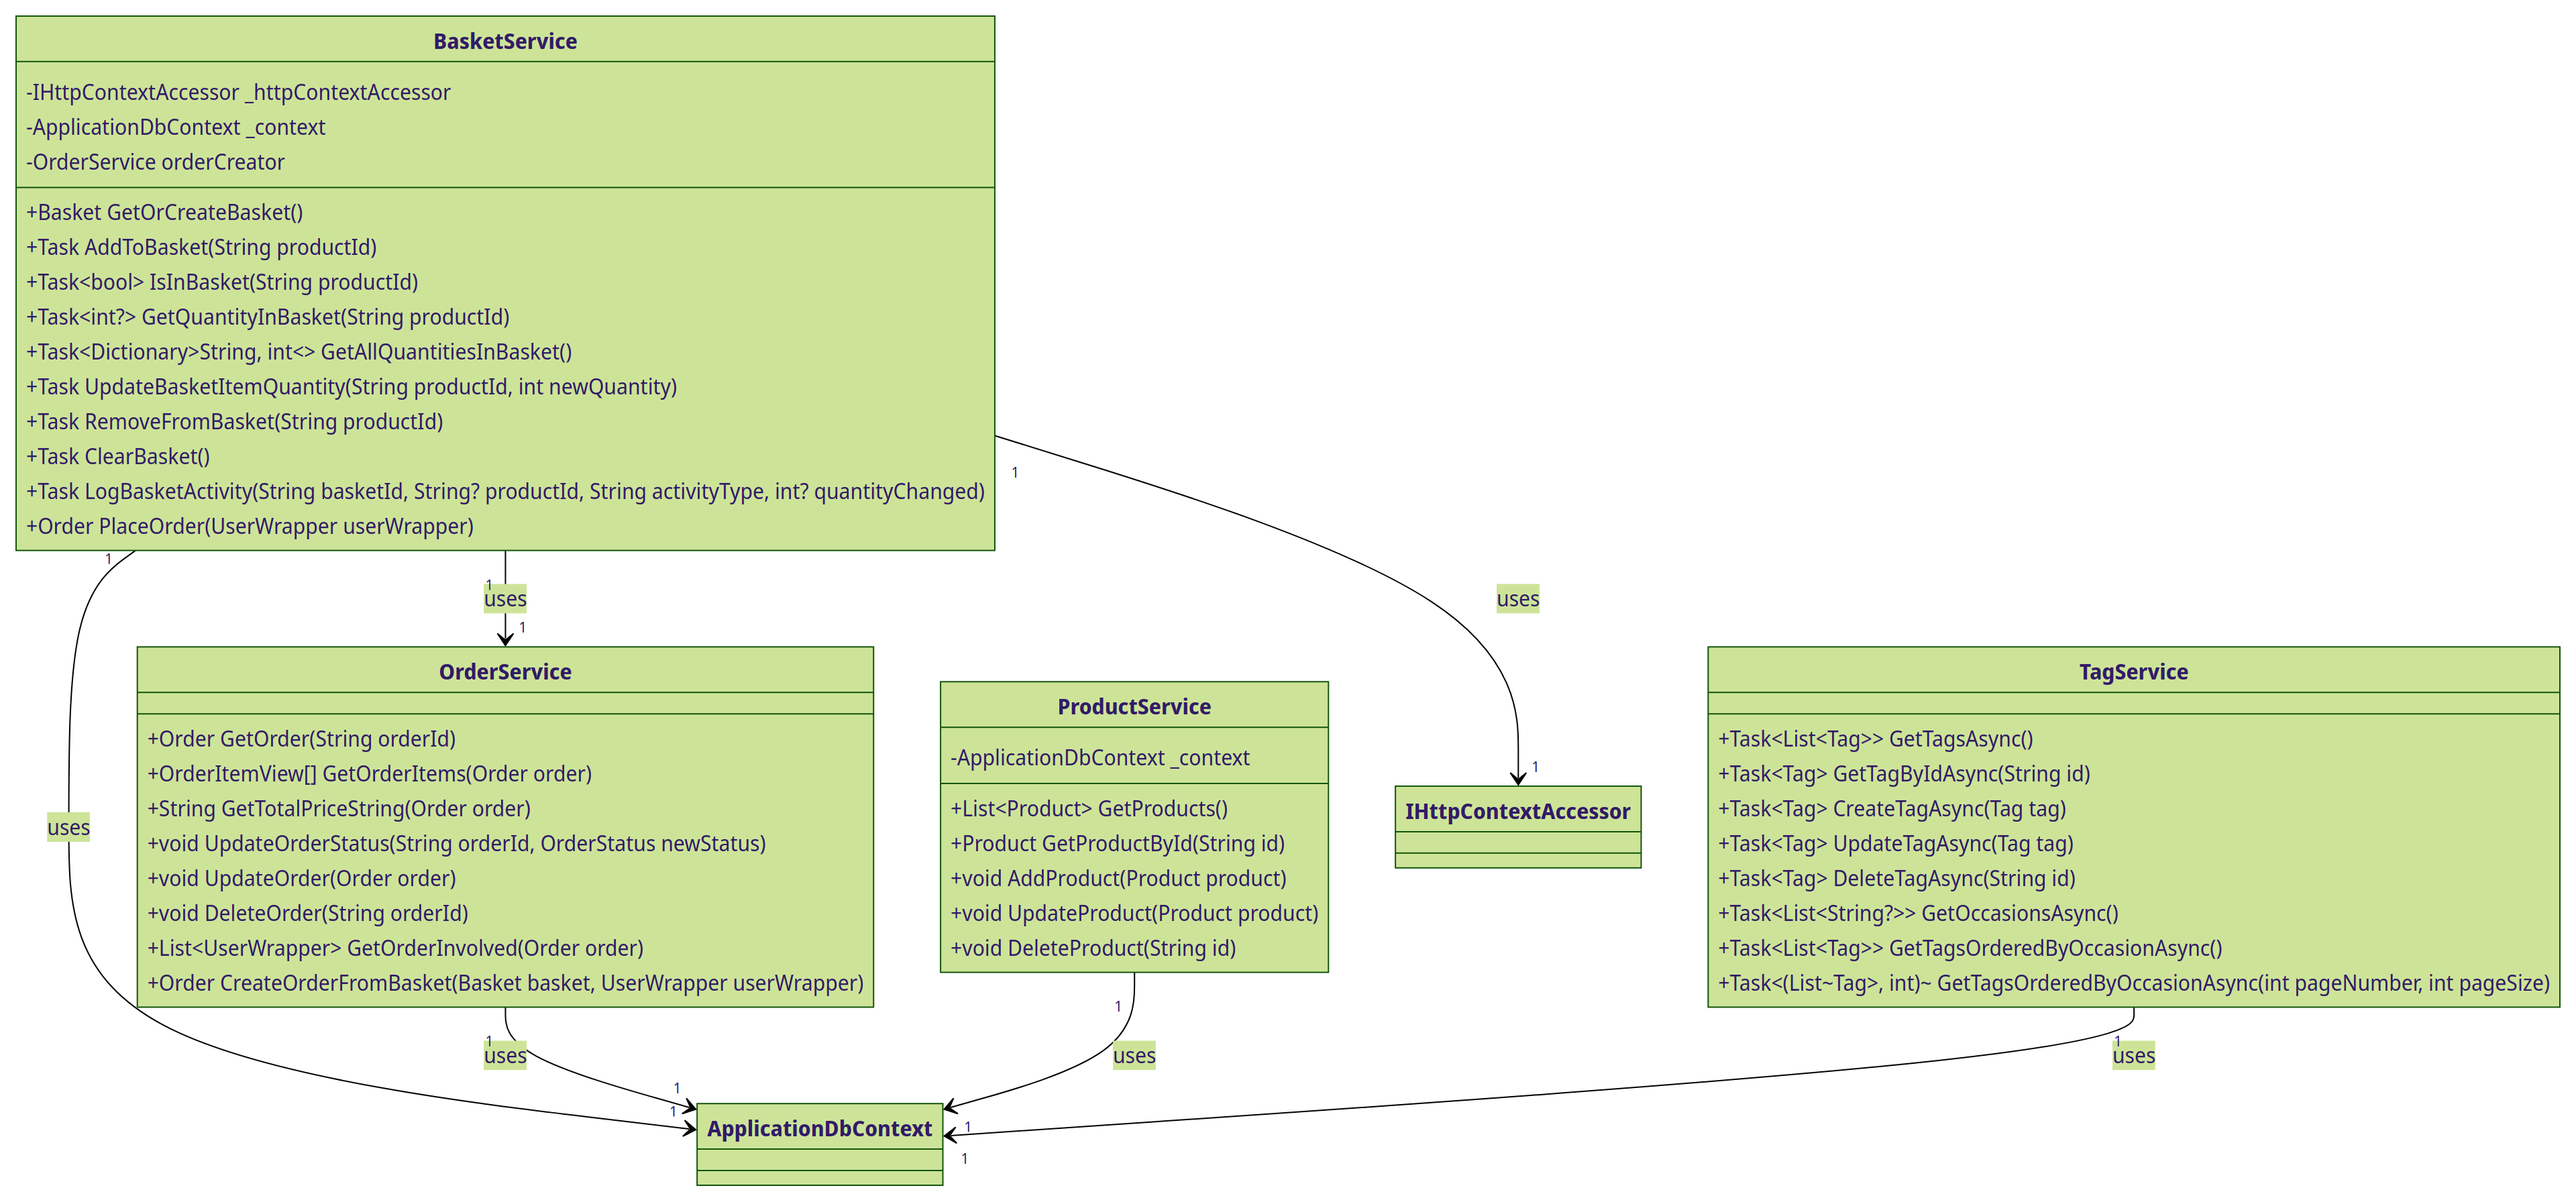
\includegraphics[width=0.8\textwidth]{figures/diagrams/dcd-main-services.png}
    \caption{Design Class Diagram - Main Services}
    \label{fig:class-diagram-main-services}
\end{figure}

\begin{figure}
    \centering
    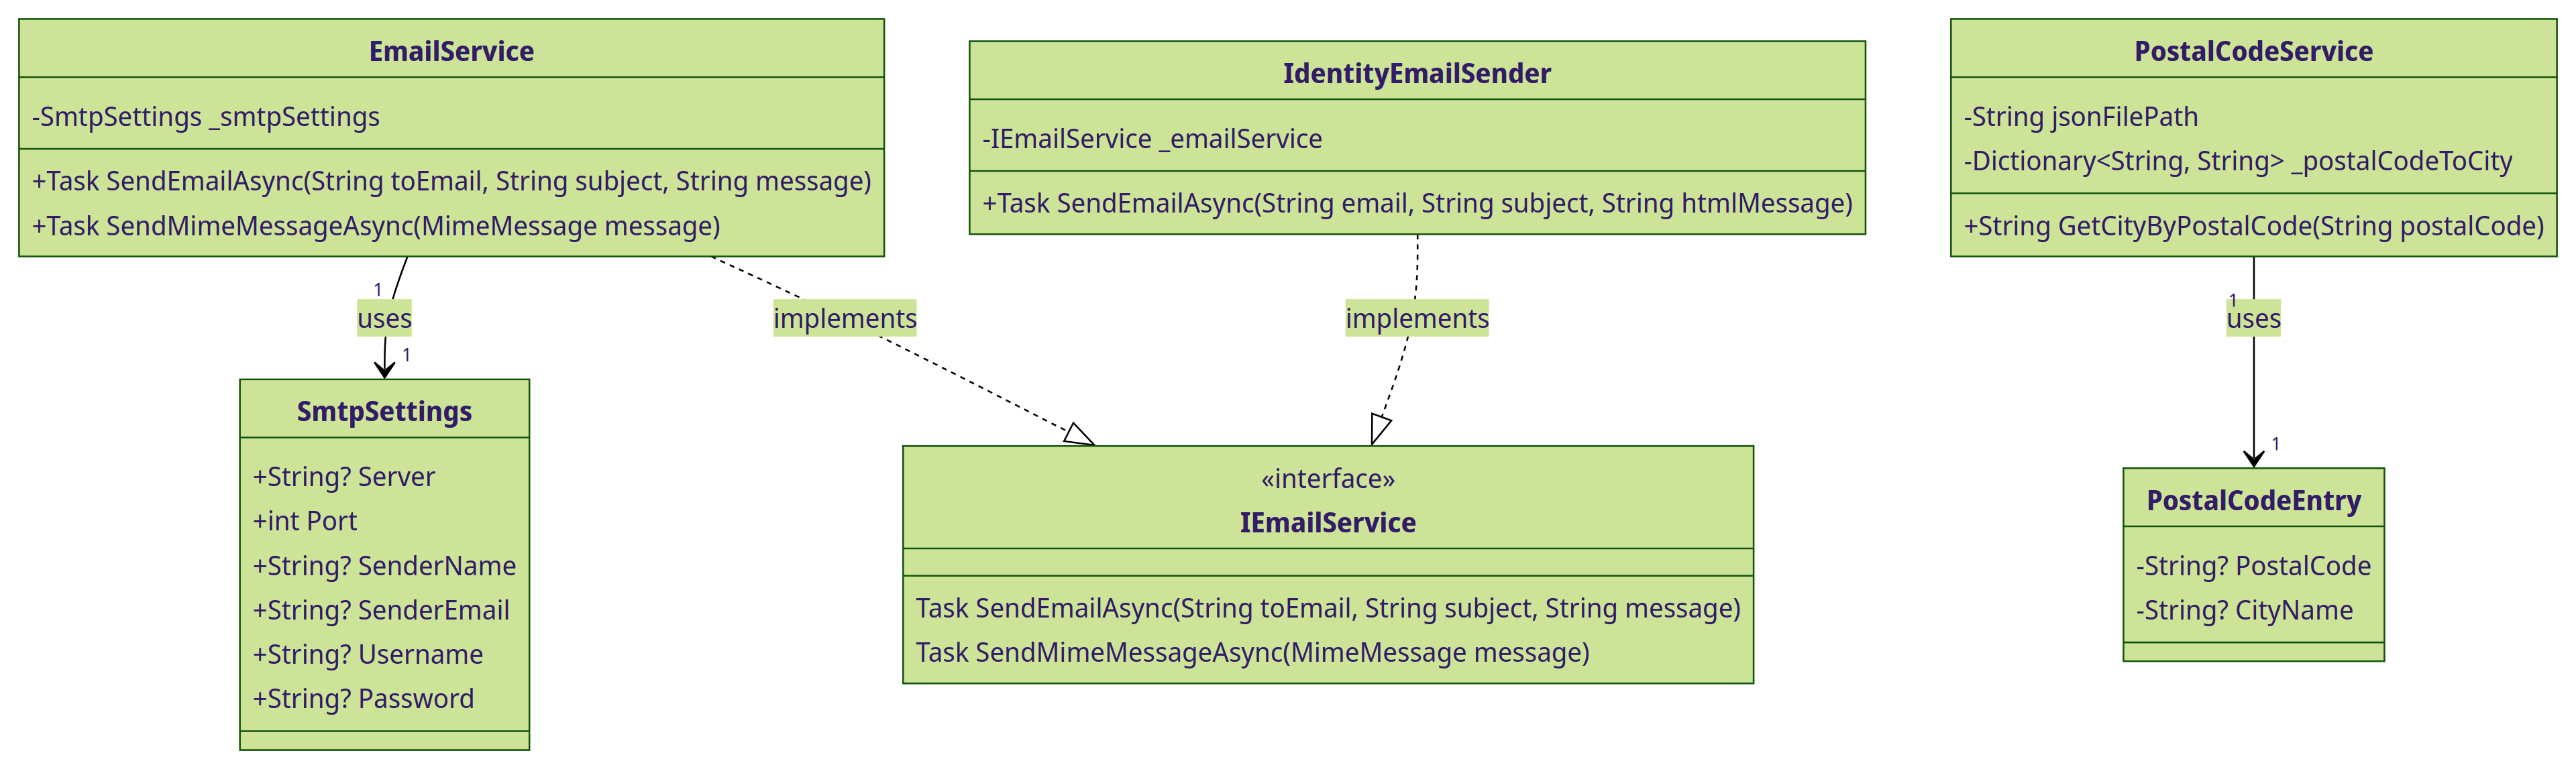
\includegraphics[width=0.8\textwidth]{figures/diagrams/dcd-aux-services.png}
    \caption{Design Class Diagram - Auxilary Services}
    \label{fig:class-diagram-aux-services}
\end{figure}
Alle modeller er vedlagt i \Cref{appendix:models} og vil ikke blive gennemgået her, grundet deres simplicitet.

\subsection{Database Design}
Viden fra \cite{connolly2023database} vil anvendes hele vejen igennem, men ikke blive citeret yderligere, da det anses for at være grundlæggende viden.

\subsection{Sekvens Diagrammer}

\section{Teknologier}

\section{Frameworks}

\section{Frameworks, Libraries and Packages}



\section{Design Patterns}

\section{Sikkerhed}

\section{Test}

\section{Dokumentation}